\documentclass{article}

\usepackage[english]{babel}
\usepackage{microtype}
\usepackage{graphicx}
\usepackage{wrapfig}
\usepackage{enumitem}
\usepackage{fancyhdr}
\usepackage{amsmath}
\usepackage{chemformula}
\usepackage{index}
\usepackage{hyperref}
\usepackage[margin=1.0in]{geometry}
\usepackage{qtree}
\usepackage{float}
\usepackage{booktabs}
\usepackage{tabularx}
\usepackage{textcomp}
\usepackage{multicol}

\begin{document}
\title{Summary: Nervous System Structure and Function}
\author{Dowland Aiello}
\date{April 13, 2020}

\maketitle
\tableofcontents
\fancyhf{}

\newpage

\section{Overview: actors and structures of the nervous system}

\subsection{Structure of the Neuron}

In contrast with the chemical message-reliant \textbf{endocrine} system,
the \textbf{nervous system} is capable of quickly conveying particular
messages to and from different actors in the body through \textbf{neurons}---
chemically and electrically signaling nerve cells. Typically, a neuron consists
of:

\begin{itemize}
	\item A \textbf{cell body} containing the nucleus and organelles
	\item Extensions that convey signals
\end{itemize}

In some cases, a \textbf{neuron} may be referred to as a \textbf{nerve}, should
it be wrapped in connective tissue.

\subsection{Structure of the Nervous System}

\begin{wrapfigure}{l}{0.4\textwidth}
	\centering
	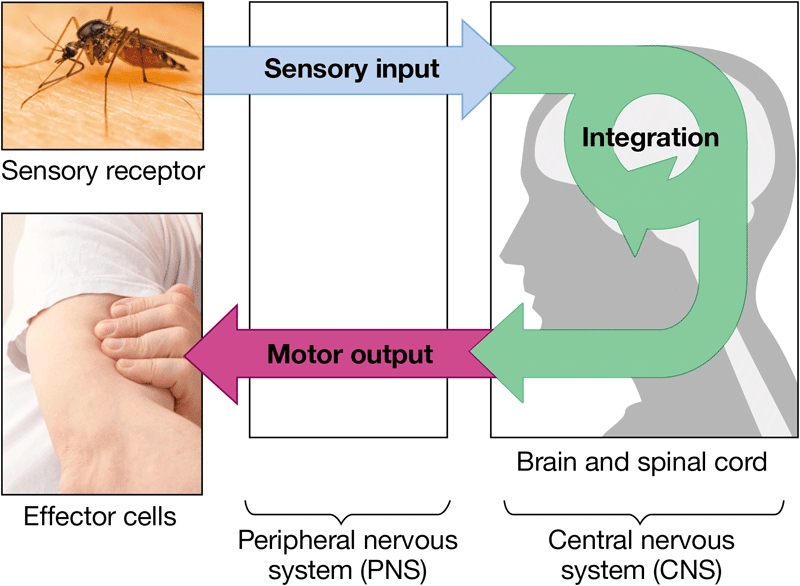
\includegraphics[width=1.0\linewidth]{goals_of_nervous_system.png}
	\caption{The three functions of the nervous system, exemplified in the human body.}
\end{wrapfigure}

The nervous system can be divided into two spatially distinct systems: the
\textbf{central nervous system (CNS)} and the \textbf{peripheral nervous
system (PNS)}. The former of the aforementioned anatomical divisions---the CNS
---is comprised by the \emph{brain} and the \emph{spinal cord} (where
applicable). The latter consists of neurons that work in conjunction with the
CNS to transmit and convey information through the body. These systems function
with the goal of providing utility with respect to three functions:

\begin{enumerate}
	\item \textbf{Sensory input}: the flow of signals from sensory receptors,
		through the PNS to the CNS
	\item \textbf{Integration}: the formation of appropriate responses to 
		certain stimuli
	\item \textbf{Motor output}: the application of responses generated through
		integration via \textbf{effector cells} (e.g., muscle, gland cells)
\end{enumerate}

In the nervous system, implementation of these three functions is achieved through
the utilization of three distinct classes of neruons: \textbf{sensory neurons},
\textbf{interneurons}, and \textbf{motor neurons}. Sensory neurons are
responsible for making data collected from the sensory receptors available to the
central nervous system. Of course, this data must \emph{integrated}. This is
achieved by the interneurons. The last of the aforementioned functions, motor output,
is provided by motor neurons, which apply responses generated through integration
via effector cells.

For example, consider the pathway of data from the outside world to effector cells
with respect to a \textbf{reflex}, such as the ``knee jerk:''

\begin{multicols}{2}
	\begin{enumerate}
		\item A tendon in the knee is tapped
		\item The quadricep muscles are stretched
		\item The stretch is detected by a sensor receptor
		\item The stretch is conveyed to the spinal cord via a sensory neuron
		\item A motor neuron in the CNS receives data regarding the ``tap''
		\item Several interneurons are made aware of the event
		\item A motor neuron signals the quadriceps to contract
	\end{enumerate}
\end{multicols}

\section{The structure of the neuron}

\subsection{Overview: neuron structure}

Neurons posess all of the cell organelles found in typical somatic cells.
However, they do posess two additionall organelles:

\begin{itemize}
	\item \textbf{Dendrites}: a network of branching extensions that convey
		information from other neurons to the given neuron
	\item \textbf{The axon}: a branching extension that connects the neuron to
		other cells, and conveys information about its consituent schwann
		cells
	\item \textbf{Glia}: supporting cells that may insulate, nourish, or
		otherwise aid in maintaining homeostasis inside a neuron
\end{itemize}

Though its appearance might suggest otherwise, the axon is generally considered
the most structurally complicated of the three aforementioned organelles, and
its structure must be addressed independently.

\subsection{The structure of the axon}

Generally, the function of the axon can be likened to that of drainage pipe:
it controls the flow of a given content---in this case, data---from the user
(i.e., axon) to the consumer of such information (i.e., other cells). This
function is achieved through the utilization of a chain of communicating cells
(the \textbf{myelin sheath}), of which there are several variants:

\begin{itemize}
	\item \textbf{Schwann cells}: carry a signal from the neuron through the axon
	\item \textbf{Nodes of Ranvier}: carry a signal from one schwann cell to
		another schwann cell, amplifying the signal non-instantaneously
		(~150 m/sec)
\end{itemize}

A common disease that affects this flow of information, and, thus, the
efficiency of information propagation via the axon is termed ``multiple
sclerosis'', and results in the degradation of the myelin sheath, and, thus,
the conductivity of a signal from the neuron to the \textbf{synaptic terminal}
which connects to various \textbf{synapses}---``connectors'', if you will, that
carry the output signal to a nearby cell. A similar, but noticeably
differentiatede behiavor termed \textbf{neuronal plasticity} describes the ability
of the brain to ``remodal'' synpatic connections between neurons. This behavior
is hypothesized to contribute to the various underlying factors describing
autism.

\section{A neuron operates on the basis of membrane charge differences}

\begin{wrapfigure}{r}{0.25\textwidth}
	\centering
	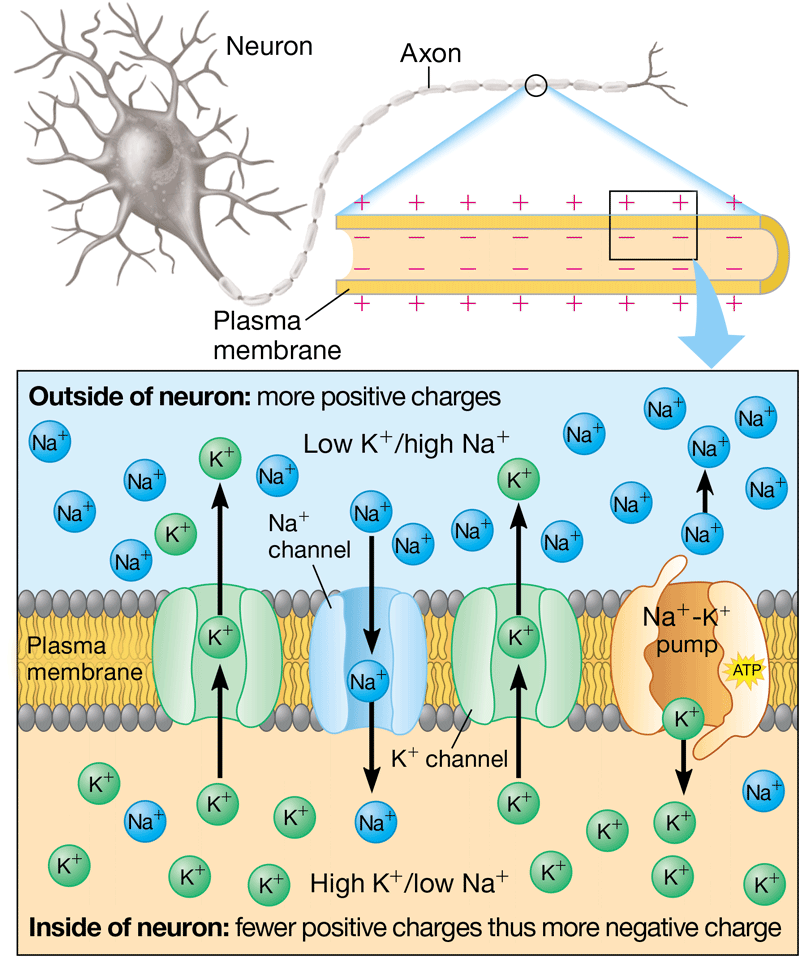
\includegraphics[width=1\linewidth]{resting_potential.png}
	\caption{How the resting potential is generated.}
\end{wrapfigure}

In order to transmit a signal from one part of the body to another, a neuron
must have the energy to do so. A \textbf{resting neuron} posesses this
\textbf{potential energy} in the form of charge differences across the membrane
of a neuron---that is, a neuron has \textbf{membrane potential}, a kind of
potential energy, which provides a neuron's capability to produce and transmit
a signal. Typically, a resting neuron posesses a negative internal charge,
relative to the charge of the surrounding fluid. This charge gradient is
generated through an equally disproportionate gradient of various ions. This
strategy of storing energy by holding separating opposite charges can be likened
to a battery, and, thus, as can a battery, the stored energy in a neuron can be
measured in terms of the neuron's \textbf{resting potential} (typically around
-70 mV).

In a neuron, the careful balance of potassium ions inside and outside of the cell
(again, there is usually a greater concentration of \ch{K+} inside the cell
than outside of the cell and a lower concentration of \ch{Na+} inside the cell
than outside the cell) is maintained through the utilization of an active
\ch{Na+}-\ch{K+} pump, wherein energy is expended in the intake of \ch{K+} and
in the expulsion of \ch{Na+}. However, active transport is not the only
membrane-bound force at play in resting potential: \textbf{ion channels} allow
\ch{K+} and \ch{Na+} to diffuse through the cell membrane, passively, through
their respective pores.

In response to \textbf{stimuli}, or any factor illiciting the generation of a
nerve signal, a neuron might expend its resting potential through a series of
electrical changes comprising an \textbf{action potential}, which is caused as
a result of rapid ion movement at various \textbf{voltage-gated ion channels}:

\begin{enumerate}
	\item The cell posesses resting potential (higher \ch{K+} concentration inside
		than outside, and a lower concentration of \ch{Na+} inside the cell than
		outside)
	\item Should the application of the stimulus be sufficient to trigger the
		neuron, the voltage of the neuron rises to the activation threshold
		(i.e., -50 mV).
	\item The action potential is triggered, resulting in a positive internal
		cell charge, with respect to the outside of the cell
	\item The voltage inside the neuron rapidly decreases
	\item The voltage inside the neuron undershoots the resting potential
	\item The voltage inside the neuron reaches the resting potential
\end{enumerate}

\begin{figure}[h]
	\centering
	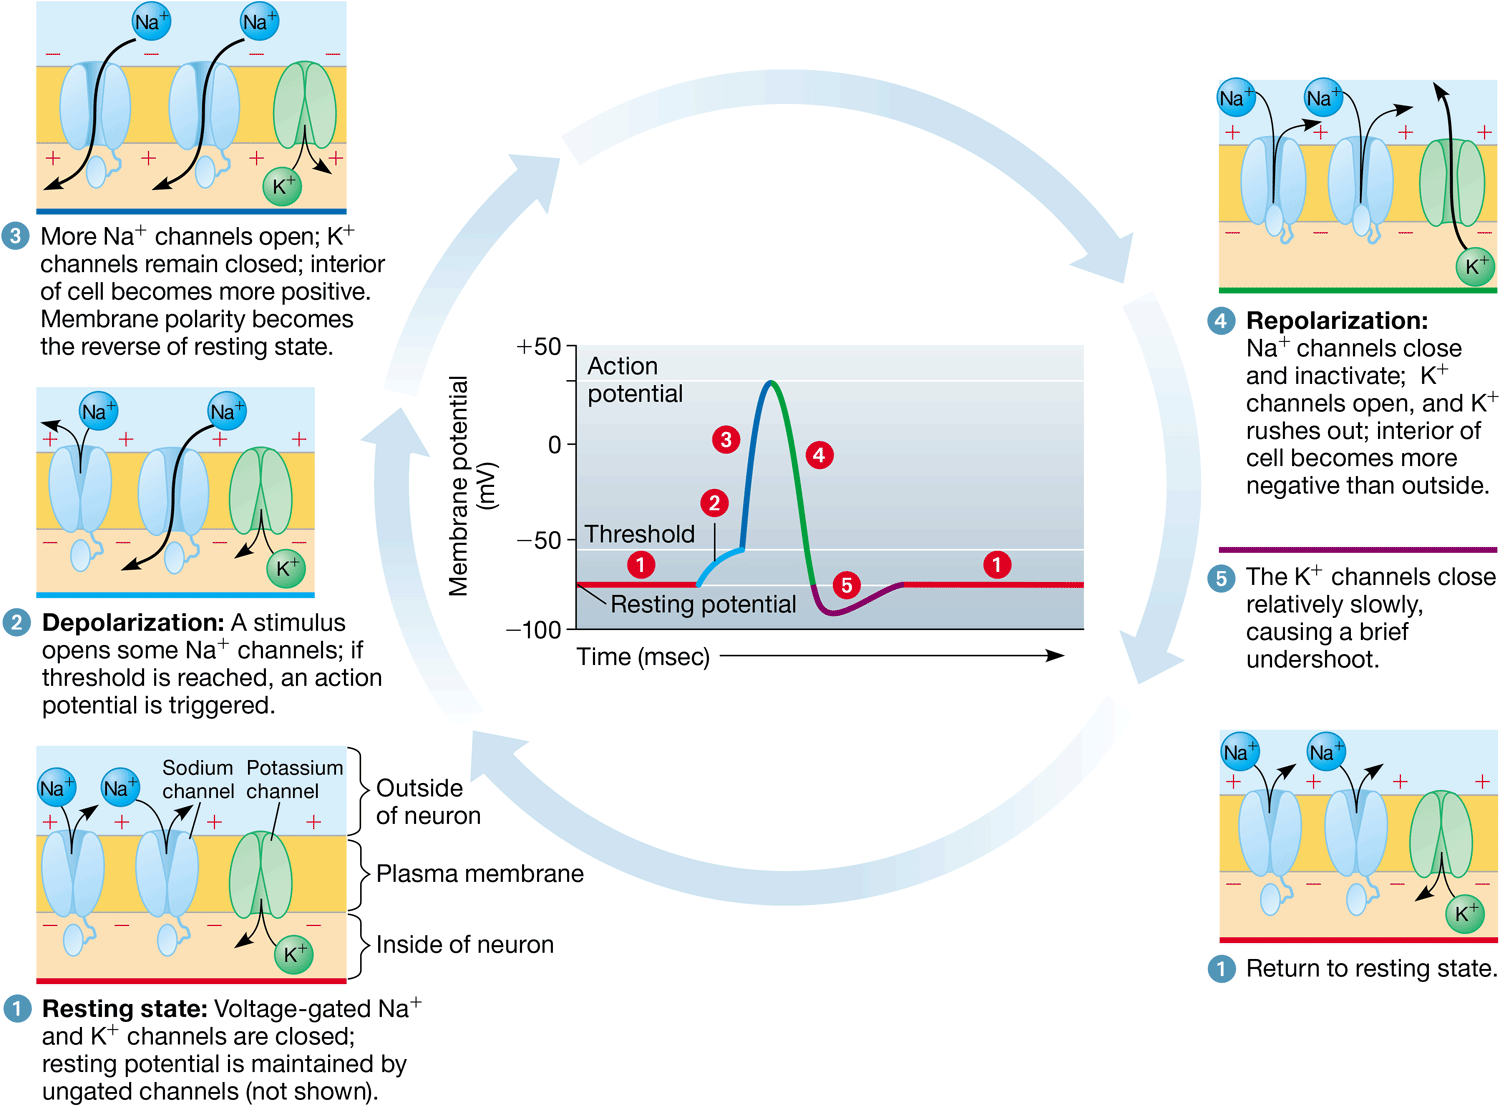
\includegraphics[width=0.8\linewidth]{depolarization.png}
	\caption{The electrical changes and ion movements in an action potential}
\end{figure}

\subsection{The continuation of action potential through the axon}

In order to be transferred from the body of the nerve cell to the synaptic
terminal, a signal must be regenerated along the axon. This action can be
likened to a chain of dominos, wherein various distinct actors change the
state of a much larger space via a ``chain reaction''. In the axon, this
``domino effect'' takes place as such:

\begin{enumerate}
	\item \ch{Na+} rushes into a Schwann cell somewhere along the axon,
		resulting in the generation of action potential
	\item \ch{K+} is expelled from the Schwann cell via diffusion, as \ch{Na+}
		remain in the cell, resulting in a decreasing action potential
	\item No action potential exists in the schwann cell
\end{enumerate}

\begin{figure}[h]
	\centering
	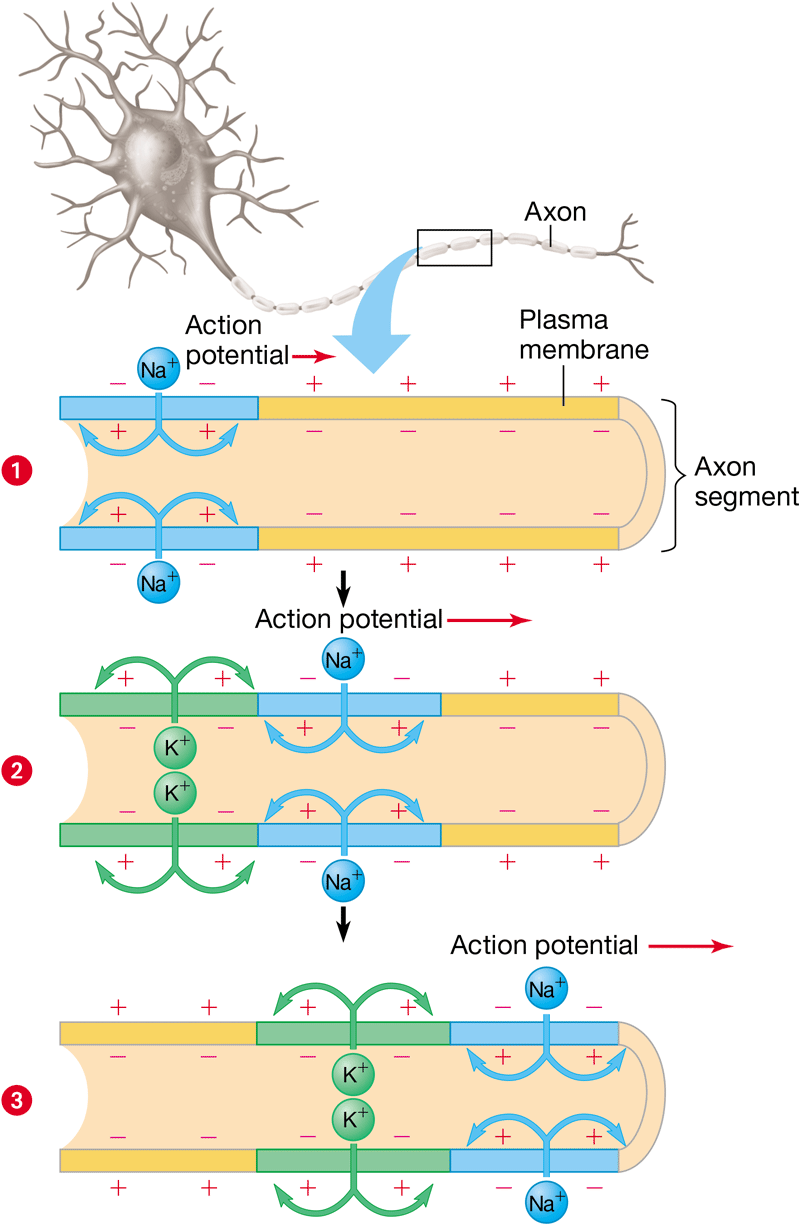
\includegraphics[width=0.5\linewidth]{action_potential_domino_effect.png}
	\caption{Propagation of the action potential along an axon}
\end{figure}

This system of cascading action potentials is not capable of back-propagation.
However, it is capable of illustrating various intensities of activation through
differing \emph{frequencies} of action potentials.

\section{The structure of a synapse}

Once a signal reaches the synaptic terminal, the signal can be conveyed via an
electrical or chemical synapse, corresponding to a neuron, effector cell, muscle
cell, or endocrine cell. The former of these two synapse types---the elecrical
synapse---operate on the basis of gap junctions, which allow for the direct
transmission of an electrical current from the neuron to a receiving cell. By
contrast, chemical synapses operate on the basis of conversion of an electrical
current to a chemical signal comprised of \textbf{neurotrasmitters}, which
induce an action potential across a synaptic cleft in the receiving cell.

\newpage

\begin{figure}[h]
	\centering
	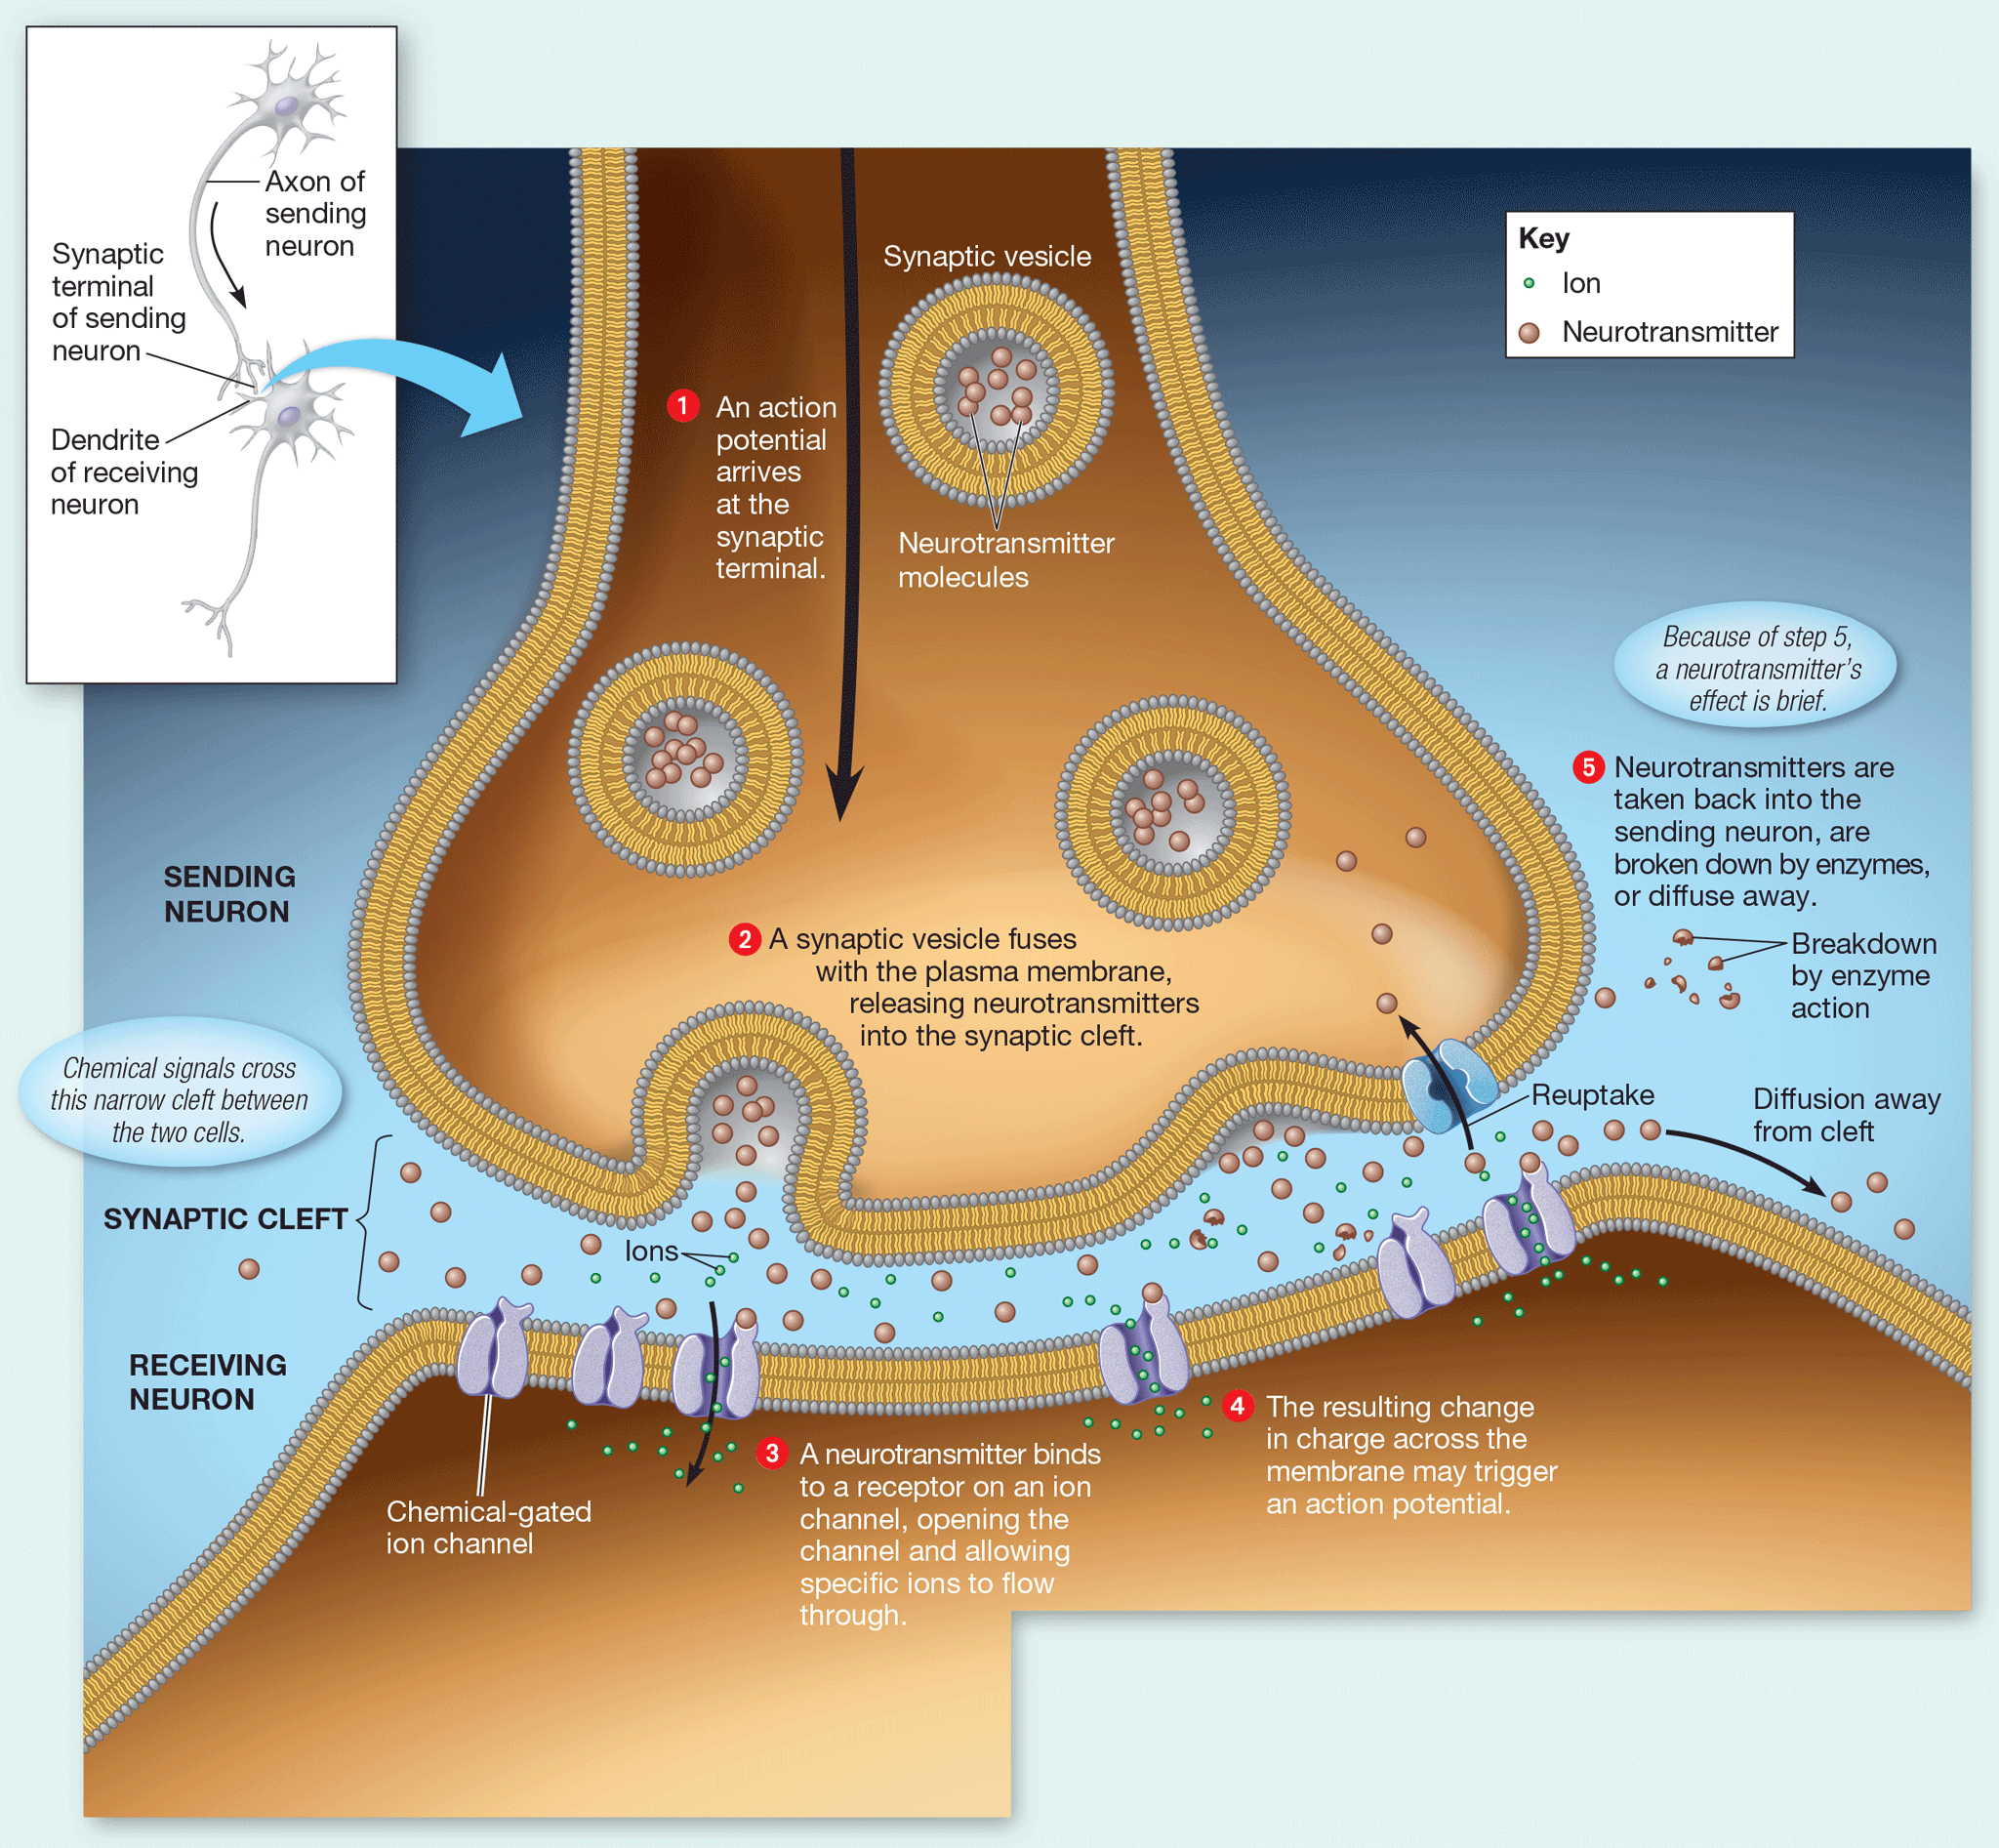
\includegraphics[width=0.75\linewidth]{synaptic_cleft.png}
	\caption{The synaptic cleft}
\end{figure}


\subsection{The structure of a chemical synapse}

A neurotransmitter that is released at a synaptic cleft acts on a receiving cell
in one of two ways: by \emph{triggering} an action potential (excitatory) or
by decreasing the likelihood of action potential developing in the receiving
cell (inhibitory).

Respectively, these outcomes are achieved through the opening of \ch{Na+} channels
and the opening of \ch{K+} release channels (i.e., in order to decrease the
probability of developing potential action in a receiving cell, \ch{Cl-} must
enter the cell, while \ch{K+} should exit). Furthermore, excitatory and
inhibitory reactions can be caused by any one of the 100 neurotransmitters
commonplace in the human nervous system: \textbf{acetylcholine}, for example, is
used to stimulate skeletal muscles, and is released by motor neurons.
The function of various neurotransmitter molecules is outlined below:

\begin{itemize}
	\item Acetylcholine: slows the rate of contraction of cardiac muscles, while
		stimulating skeletal muscles
	\item Botulinum toxin: inhibits the release of acetylcholine
	\item Glutamate: aids in the formation of long-term memory
	\item Gamma aminobutyric acid: serves as a neurotransmitter in amny inhibitory
		CNS synapses
	\item Serotonin, dopamine: affect sleep, mood, attention, and learning
\end{itemize}

\section{Systems of the nervous system}

\subsection{The central nervous system}

In all vertebrates, the \textbf{brain} and \textbf{spinal cord} comprise the
central nervous system (CNS). The former of these composing structure, the
\textbf{brain} aids in maintaining homeostasis by integrating sensory data.
The \textbf{spinal cord}, on the other hand, allows for the transmission of
data from the PNS to the brain.

\begin{figure}[h]
	\centering
	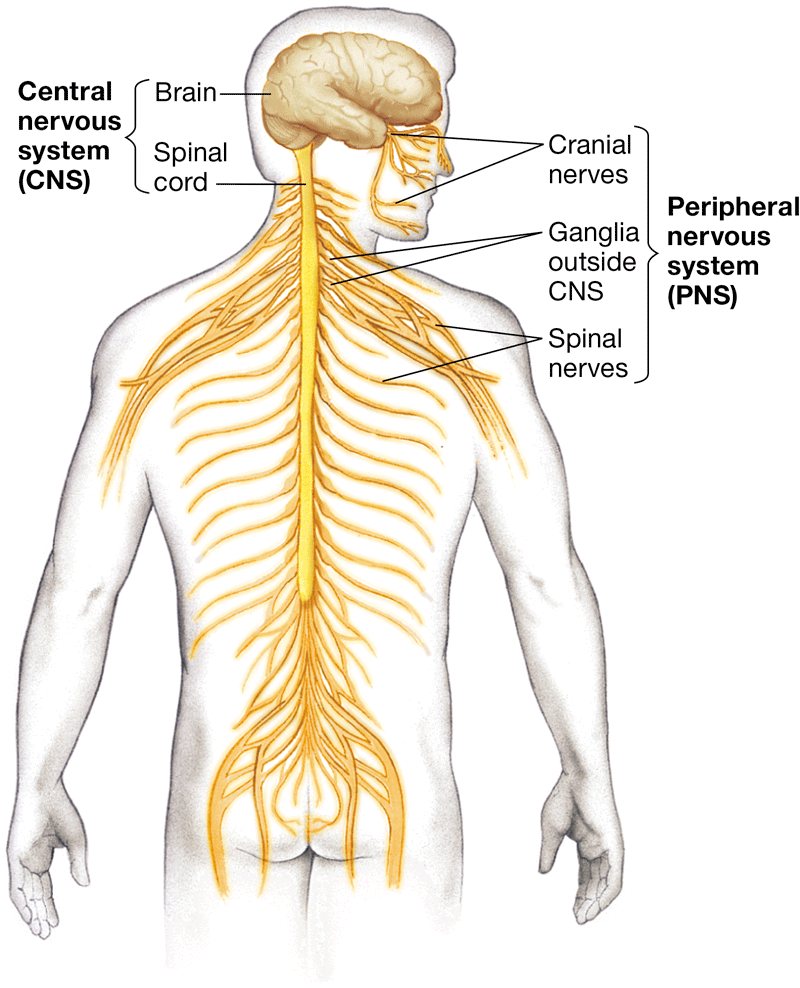
\includegraphics[width=0.7\linewidth]{nervous_system.png}
	\caption{A vertebrate nervous system}
\end{figure}

Furthermore, the functionality of the central nervous system is maintained
through various blood vessels (termed the \emph{blood-brain barrier}), which
allow for the propagation of nutrients and oxygen into the brain. Through
the utilization of this system, \textbf{cerebrospinal fluid}---nourishing fluid
that circulates through the central canal---is able to be produced via the
filtration of blood passed to this region. In addition to the cerebrospinal
fluid, two types of fluid circulate through these organs:

\begin{itemize}
	\item \textbf{White matter} composed of axons and myelin sheaths
	\item \textbf{Gray matter} composed of neuron cell bodies
\end{itemize}

\subsection{The periphery nervous system}

\begin{wrapfigure}{r}{0.3\textwidth}
	\centering
	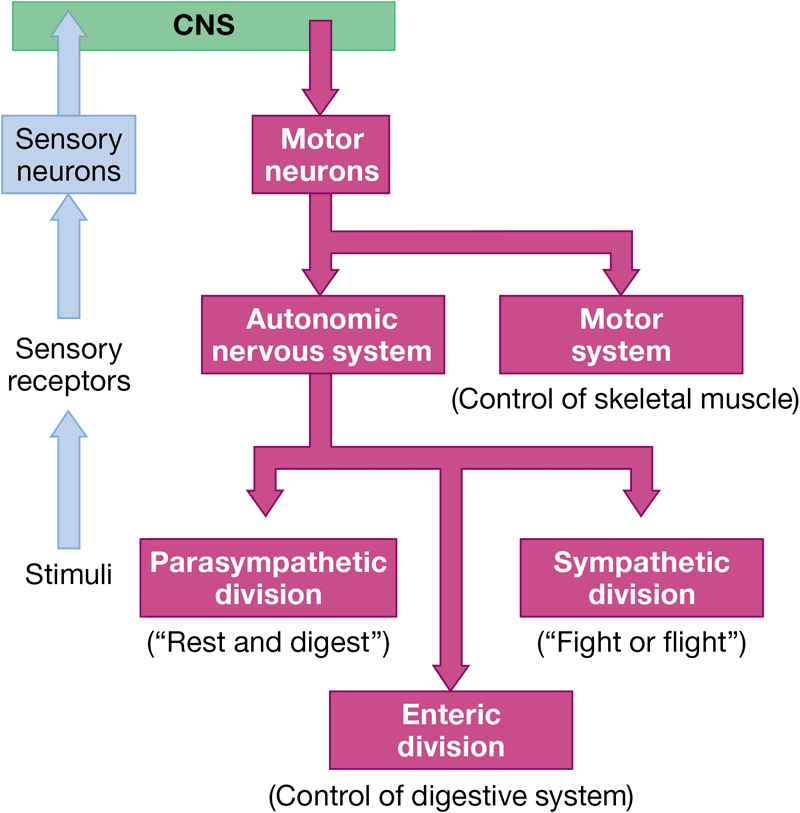
\includegraphics[width=0.9\linewidth]{cns_out_in_flow.png}
	\caption{Divisions of the PNS in vertebrates}
\end{wrapfigure}

In vertebrates, the PNS is divided into sensory neuron groups, which convey data
to the central nervous system, and motor neuron groups. In contrast with sensory
neurons which take information from the periphery of the body to the central
nervous system (i.e., in an outward-in fashion), motor neurons transmit information
in an outward-in manner---that is, once a signal has been ``transformed'' or
``integrated'', the signal can be sent to an effector cell.

Furthermore, once data has been integrated, it must be sent from the CNS to the
PNS, and to one of the types of motor neurons: a \textbf{motor system} neuron
handling generally voluntary actions, or an \textbf{autonomic nervous system}
neuron dealing with involuntary actions. These two systems are asynchronous,
and cooperate in order to maintain homeostasis.  On an even more
physiologically detailed basis, one may differentiate between the
\textbf{parasympathetic}, \textbf{sympathetic} and \textbf{enteric} divisions
within the autonomic nervous system. The function of each of these divisions
is defined as such:

\begin{itemize}
	\item \textbf{Parasympathetic division}: stimulate the digestive organs,
		preparing the body to conserve or gain energy
	\item \textbf{Sympathetic division}: inhibits the function of the digestive
		organs temporarily, preparing the body for energy-consuming activities
	\item \textbf{Enteric division}: aid in the secretion of hormones that
		control peristalsis---the constriction and relaxation of the intestine
\end{itemize}

\subsection{The development of the brain in vertebrates}

In vertebrates, the neural tube gives rise to three divisions that are molded
into the various structures present in the developed brain: the 
\textbf{forebrain}, the \textbf{midbrain} and the \textbf{hindbrain}.

The first of these divisions, the forebrain gives rise to both the
\textbf{cerebrum} and the \textbf{dinecephalon}. The midbrain, on the other
hand, is aptly described as simply the ``midbrain''. Finally, the hindbrain
develops in the form of the \textbf{pons}, \textbf{cerebellum} and the
\textbf{medulla oblongata}.

\section{The brain}

\subsection{The structures of the brain}

As can the nervous system, the brain can be divided into several function
compartments: the \textbf{forebrain}, the \textbf{midbrain} and the
\textbf{hindbrain}.

As can each of the remaining segments of the brain, the hindbrain can be
further divided into various constituent components:

\begin{enumerate}
	\item The \textbf{medulla oblongata} and the \textbf{pons}: transfer data
		from the CNS---the spinal cord, specficially---to the forebrain, and
		maintain autonomic bodily functions
	\item The \textbf{cerebellum}: coordinates movement and balance with
		respect to information obtained from the sensory organs dealing with
		the position of joints and the length of muscles in the body (e.g.,
		hand-eye coordination)
	\item The \textbf{brainstem}: deals with the integration and transfer to the
		forebrain of sensory data
\end{enumerate}

In contrast with the hindbrain, the forebrain is generally concerned with the
maintanence of much higher-level body functions, and is composed of the
following structures:

\begin{itemize}
	\item The \textbf{cerebrum}: deals with the mobility of each side of the
		body---though mobility is generally delegated to one of the two
		\textbf{cerebral hemispheres} within the cerebrum (i.e., the right
		cerebral hemisphere is responsible for the mobility of the left side
		of the body, while the right side is responsible for the right side of
		the body). The cerebrum is the largest structure in the brain.
	\item The \textbf{thalamus}: relays sensory information to the cerebral
		cortex after sorting data into categories.
	\item The \textbf{hypothalamus}: responsible for the body's ``biological
		clock'', and exerts control over the pituitary gland, thus giving it
		responsibility with respect to the fight-or-flight response, thirst,
		hunger, and mating behaviours.
	\item The \textbf{pituitary gland}
\end{itemize}

\begin{figure}[h]
	\centering
	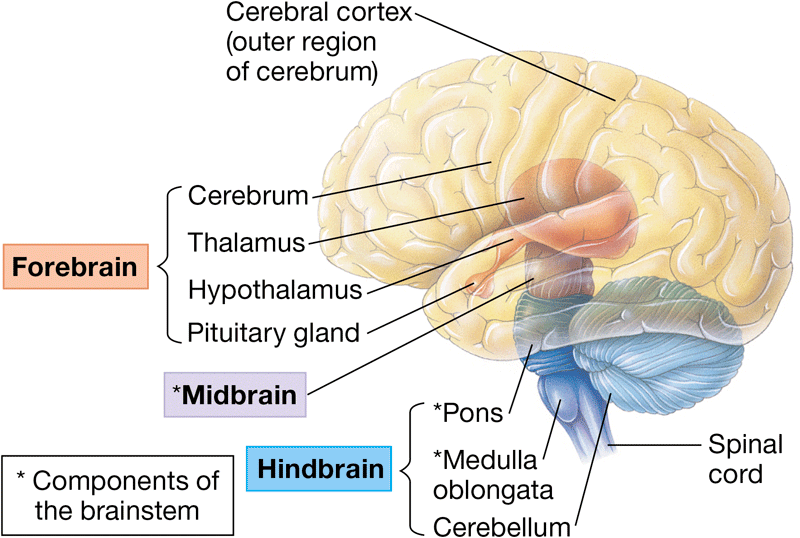
\includegraphics[width=0.45\linewidth]{basic_brain_structure.png}
	\caption{The basic structure of the brain}
\end{figure}

\subsection{The cerebral cortex}

Structurall, the cerebral cortex bears similarity to the cerebrum in its
division into a right and left side, connected by the \textbf{corpus callosum},
each of which are further divided into quadrants named according to a nearby
placemarker (i.e., a bone). Functionally, however, the cerebral cortex could
not be more dissimilar to the cerebrum. In other words, the cerebral cortex is
responsible for the proper expression of the most advanced behaviors exhibited
by humans: personality, metacongnitive ability, etc\ldots, each of which is
dealt with by the respective lobe (i.e., according to recent research, it
appears that the left hemisphere is more suited towards logical operations, while
the right hemisphere deals with patterns, relations, and nonverbal thinking).

\bigbreak{}

\begin{figure}[h]
	\centering
	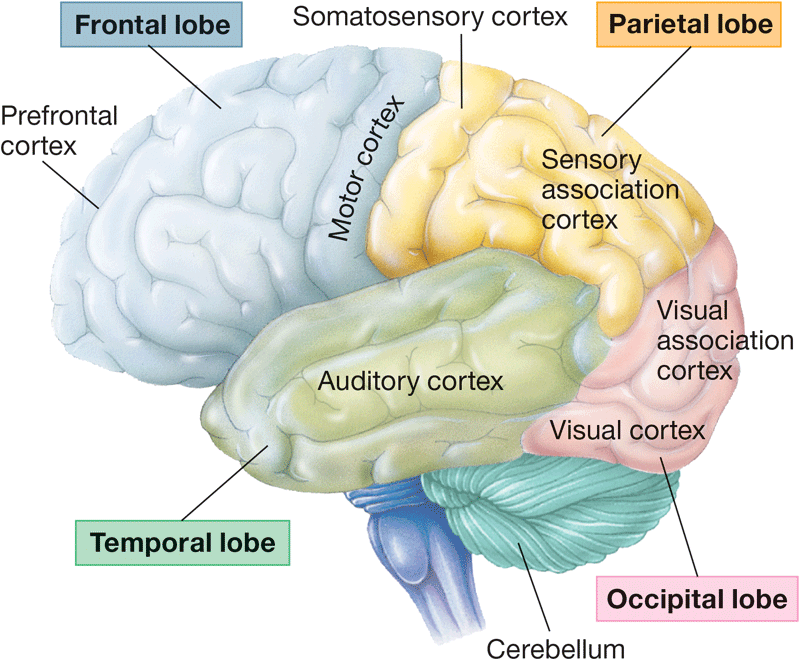
\includegraphics[width=0.35\linewidth]{lobes.png}
	\caption{The various lobes in the cereberal cortex}
\end{figure}

\subsection{The limbic system}

The limbic system is composed of various parts of the thalamus and hypothalamus,
and is responsible for human emotion, motivation, and memory. In addition to the
aforementioned segments of the thalamus and hypothalamus, the amygdala and
hippocampus aid in the formation of emotional memories and the formatio and
recollection of general memories, respectively. In the case of short-term
memory formation, for example, a ``link'' forms in the hippocampus to information
stored in the cerebral cortex. Long-term memories, on the other hand, are comprised
by connections in the cerebral cortex, rather than the hyppocampus.

\bigbreak{}

\begin{figure}[h]
	\centering
	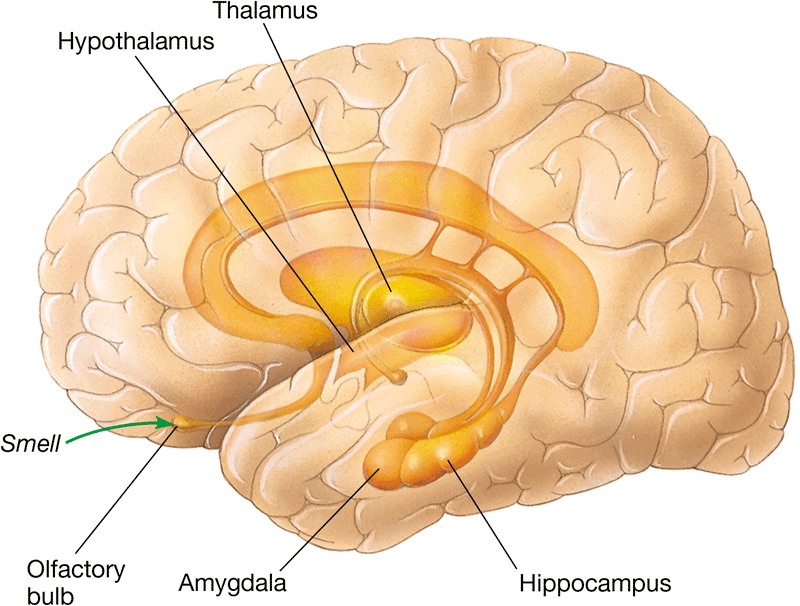
\includegraphics[width=0.7\linewidth]{limbic_system.png}
	\caption{The limbic system}
\end{figure}

\end{document}
